\section{Study 14: magnesium in acute myocardial infarction}\label{sec:study14}
Theorem J was proved for injected records and tested on simulated sources (\cref{sec:study13}). Its band identity needs no latent
model, so it can be applied to real published evidence. Study 14 applies it to a well-known case: intravenous magnesium after
myocardial infarction, where small trials and an overview \cite{Teo1991} suggested a large mortality benefit, LIMIT-2 \cite{Woods1992}
supported a benefit, and ISIS-4 \cite{ISIS41995} found none \cite{EggerDaveySmith1995}. The question is not whether the
lab's latent two-type model holds for patients; aggregate trial tables cannot identify patient-level types. It is narrower:
\emph{before ISIS-4, did the evidence settle the treatment decision, or only the statistics?}

\paragraph{Design and registration.} The study was registered and frozen with SHA-256 before any trial count was extracted
(\texttt{engine/\allowbreak study14\_magnesium/\allowbreak PREREG\_study14.md}). It could not be blind: the registration states what
the author knew of the history and which predictions are anchors rather than tests. The trials are grouped into three sources: $S$, the
seven small trials of the 1991 overview; $L$, LIMIT-2; $I$, ISIS-4. Analysis sets are unions of trials, never of pooled estimates:
before ISIS-4 ($S\cup L$, the pool of the 1993 overview \cite{YusufTeoWoods1993}) and after it ($S\cup L\cup I$). Each trial gives a log
odds ratio with its binomial variance, and sources are pooled by fixed-effect inverse variance. With $\pi$ the inverse-variance
share of $S$ and $Z_S$ its standardised contrast with the rest, the pooled estimate moves away from the rest by exactly
$Z_S\sqrt{\pi/(1-\pi)}$ pooled standard errors (\cref{thm:J}(2)). Hence the \emph{observed non-rejection band}
\[
B=1.96\sqrt{\pi/(1-\pi)} :
\]
of all placements of $S$ that a $1.96$ contrast test would not reject, none moves the pool by more than $B$ standard errors. This is the
special case $c_s=1.96$, $\beta=\tfrac12$ of \cref{thm:J}(2), read as a statement about the evidence, not as the theorem's
exposure-risk guarantee. Treatment is justified if the absolute reduction in mortality exceeds $h\in\{0,0.5,1,2\}$ percentage points at a
reference control risk $p_0=0.10$ (sensitivity $0.07$), mapped exactly to a log-odds threshold. With $M$ the margin to that threshold in
pooled standard errors, the evidence is \emph{statistically settled} for treatment when $M>1.96$, and \emph{decision-settled} when
$M-B>1.96$; against treatment, $M<-1.96$ and $M+B<-1.96$. The hiding segment and $n^*$ are not used: trial data do not have the lab's
shape.

\paragraph{Data.} The overview's own trial table was not reachable, so the counts come from Egger, Davey Smith and Altman's tabulation
\cite{EggerSmithAltman2001} (disclosed as a deviation). The seven small trials reproduce the overview's reported totals exactly: $25$ of
$657$ deaths with magnesium and $53$ of $644$ without.

\begin{table}[!htbp]\centering\small
\begin{tabular}{lcccccc}\toprule
 & pooled OR & $Z_S$ & $\pi$ & $B$ & $M$ at $h=0$ & $M-B$\\\midrule
1991 ($S$) & $0.45$ (Peto) & & & & & \\
before ISIS-4 ($S\cup L$) & $0.67$ & $-1.50$ & $0.23$ & $1.08$ & $3.16$ & $2.08$\\
after ISIS-4 ($S\cup L\cup I$) & $1.03$ & $-2.98$ & $0.01$ & $0.23$ & $-1.01$ & $-1.24$\\\bottomrule
\end{tabular}
\caption{Study 14: the source $S$ of small trials, its contrast, share and band, and the margin at $h=0$ ($p_0=0.10$).}\label{tab:study14}
\end{table}

\paragraph{Results.} Five of six predictions held and the main test failed, narrowly.
\begin{itemize}
\item M1 (reproduction): the Peto odds ratio of the seven trials is $0.450$, the overview's $0.45$.
\item M2 (anchor): before ISIS-4 the evidence was statistically settled for treatment at $h=0$.
\item M3 (test) \emph{failed}: it was also decision-settled at $h=0$, since $M-B=2.08>1.96$. A small-trial source that no contrast
  test would flag could not, alone, overturn ``magnesium lowers mortality at all''. The margin is $0.12$ standard errors.
\item M4 (test): the small trials were not flagged against LIMIT-2 ($|Z_S|=1.50$).
\item M5 and M6 (anchors): after ISIS-4 the evidence is decision-settled against treatment for every $h\ge0.5$ and unsettled at $h=0$,
  and ISIS-4 flags the small trials ($|Z_S|=2.98$).
\end{itemize}

\paragraph{What the gradient shows.} The registered outputs show the distinction doing real work (\cref{fig:magnesium}(b)). Before
ISIS-4 the evidence was statistically settled for treatment at $h=0.5$ and $1$ percentage points, yet decision-settled at neither:
for every clinically meaningful threshold, an unflagged small-trial source was enough to undo the verdict. The one settled verdict, at
$h=0$, was fragile: dropping any one of three of the seven trials undoes it (\cref{fig:magnesium}(c)). Exploratory analyses after the
run, not registered, agree. An Egger-type regression does not flag the trials before ISIS-4 ($p=0.17$) and does after ($p=0.018$);
neither result identifies publication bias. LIMIT-2 alone gives $M=2.04$ at $h=0$ and is unsettled from $h=0.5$.

\paragraph{What it does not show.} The band models one shifted source. ISIS-4 also disagreed with LIMIT-2 (odds ratio $0.74$), and no
single-source band covers that. The tables cannot separate heterogeneity (the small trials sampled a different clinical context) from
selection (they are a biased sample of the same one): both appear as the same source shift, and a contrast measures disagreement, not
its cause. The study does not claim that ISIS-4 verifies any theorem.

\begin{figure}[!htbp]\centering
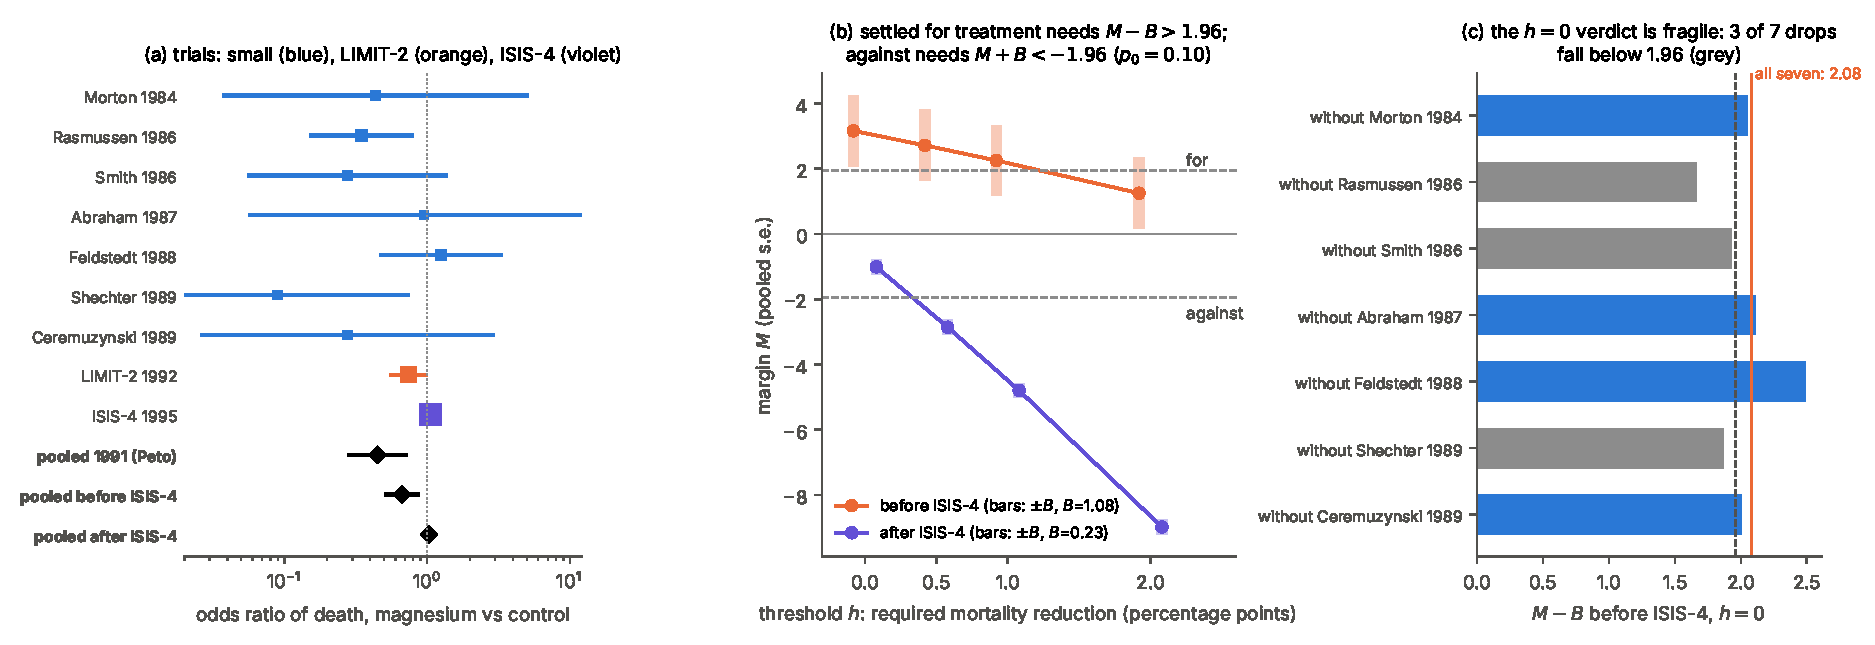
\includegraphics[width=\linewidth]{fig_magnesium.pdf}
\caption{Study 14. (a) The trials and the three pools. (b) The margin $M$ at each threshold before and after ISIS-4, with bars of
$\pm B$: before ISIS-4 only $h=0$ clears $1.96$ after the band. (c) Leave-one-out within the small trials before ISIS-4: three of seven
drops take the $h=0$ verdict below $1.96$.}\label{fig:magnesium}
\end{figure}
